\begin{mainquestion}{cascade}{Cascaded CD and CG Stages}

Consider cascading a common-drain and a common-gate stage, each of which has $g_m = 5\,\text{mS}$ and $r_o$ large enough to be ignored.

\begin{center}
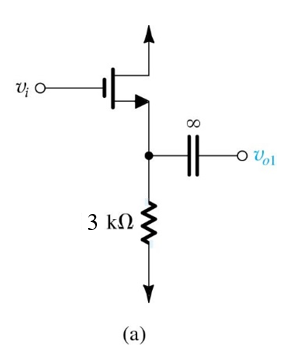
\includegraphics[width=2.5in]{cd.png}\qquad
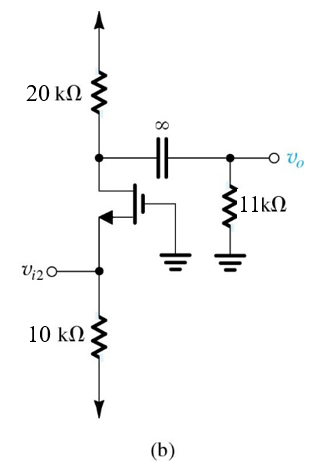
\includegraphics[width=2.5in]{cg.png}
\end{center}

\begin{partquestion}{cdgain}{Find the voltage gain $\frac{v_{o1}}{v_{i}}$ of the CD amplifier and its output resistance $R_{o1}$.}
\begin{answer}
The small signal model equivalent of this common drain stage is shown below:

\begin{center}
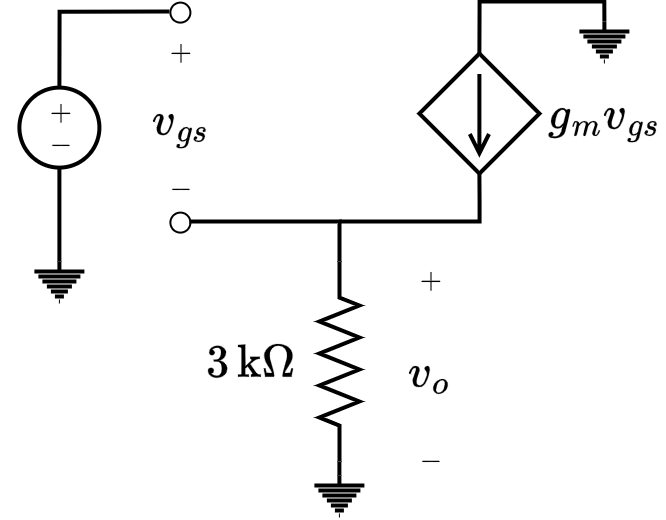
\includegraphics[width=2.5in]{sscd.png}
\end{center}

Neglecting channel length modulation ($r_o \rightarrow \infty$), the gain of the common-drain stage is:

\begin{align*}
v_{gs} &= v_i - v_{o1} \\
v_{o1} &= g_m v_{gs} R_s = g_m (v_i - v_{o1}) R_s \\
A_v &= \frac{v_{o1}}{v_i} = \frac{g_m R_S}{1 + g_m R_S} = \frac{(5)(3)}{1 + (5)(3)} = 0.9375
\end{align*}

We note this is the same form as in the lecture notes, but when $R_S$ is considered, it acts in parallel with $r_o$ , that is, ($r_o \parallel R_S$ ). However, because $r_o \rightarrow \infty$ , only $R_S$ remains, effectively taking the place of $r_o$.

The output resistance of the circuit can be found by shorting the input signal and applying a test source at the output terminals, as seen in the image below. The output resistance can be calculated by finding the current on the test voltage source.

\begin{center}
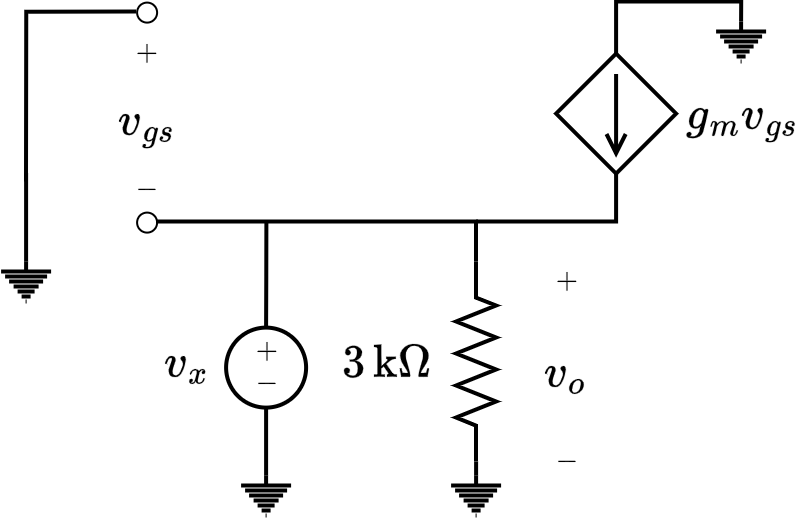
\includegraphics[width=2.5in]{rthcd.png}
\end{center}

We have:
\begin{align*}
    v_{gs} &= 0 - v_{x} \\
    i_{x} - \frac{v_{x}}{R_S} &= g_m v_{gs} = - g_m v_{x} \\
    R_{o1} &= \frac{v_{x}}{i_{x}} = \frac{R_S}{1+ g_m R_S} = \frac{3}{1 + (5)(3)} = \qty{0.188}{\kilo\ohm} = 188\Omega
\end{align*}

\end{answer}
\end{partquestion}

\begin{partquestion}{cgopenocgain}{Find the open-circuit voltage gain $\frac{v_{o}}{v_{i2}}$, the input resistance, and the output resistance of the CG amplifier.}
\begin{answer}

The small signal model equivalent of this common gate stage is shown below:

\begin{center}
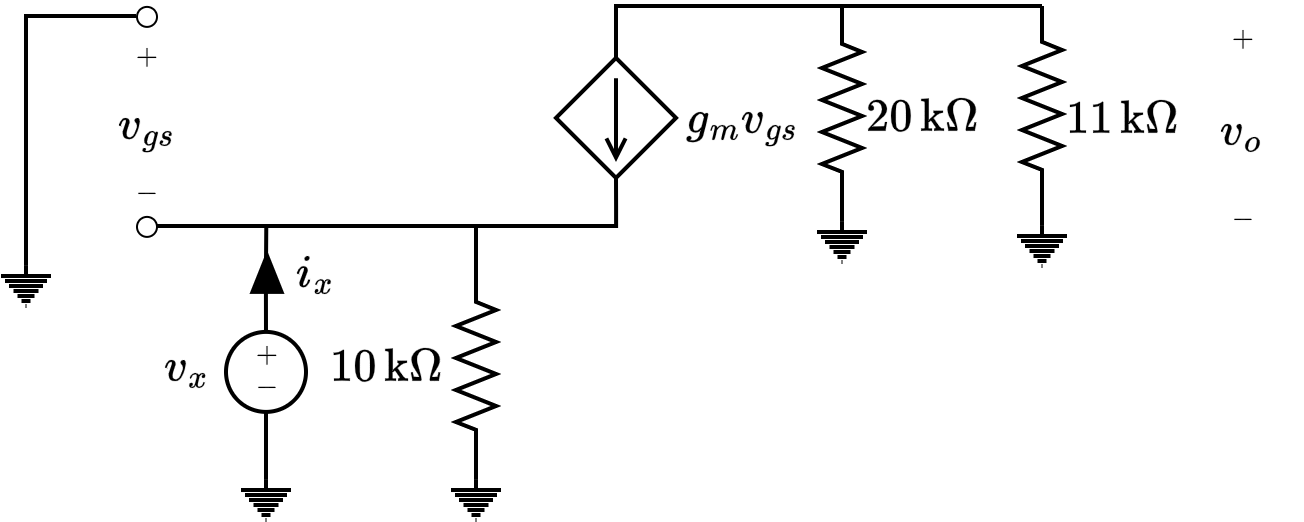
\includegraphics[width=3.5in]{sscg1.png}
\end{center}

Neglecting channel length modulation, the gain of the common gate stage:

\begin{align*}
    v_{gs} &= 0 - v_{i2} \\
    v_o &= -(R_D \parallel R_L) g_m v_{gs} = (R_D \parallel R_L) g_m v_{i2}
\end{align*}

Recall we let $R_L \rightarrow \infty$ when considering open-circuit gain, so the circuit looks like:
\begin{center}
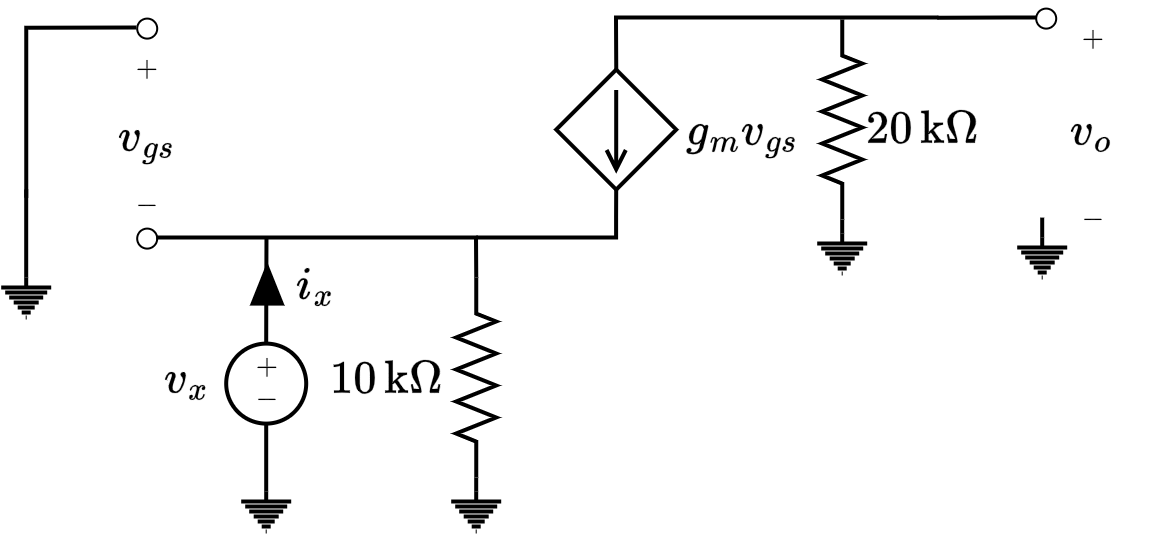
\includegraphics[width=3.5in]{sscg1b.png}
\end{center}
The gain is calculated as:
\begin{align*}
    A_{vo} &= \left.\frac{v_o}{v_{i2}}\right|_{R_L \rightarrow \infty} \\
    &= (R_D)g_m \\
    &= (20)(5) \\
    &= 100
\end{align*}


The input resistance can be found by calculating the current coming out of the input source:

\[
i_{i2}=\frac{v_{i2}}{R_{S}}-g_{m}v_{gs}=\frac{v_{i2}}{R_{S}}+g_{m}v_{i2} 
\]

And therefore:
\[
R_{i2}=\frac{v_{i2}}{i_{i2}}=\frac{1}{\frac{1}{R_{S}}+g_{m}}=\frac{1}{\frac{1}{10}+5}= \qty{0.196}{\kilo\ohm}=196\ \Omega
\]

The output resistance of the circuit can be found by shorting the input signal and applying a test source at the output terminals, as seen in the image below. 

\begin{center}
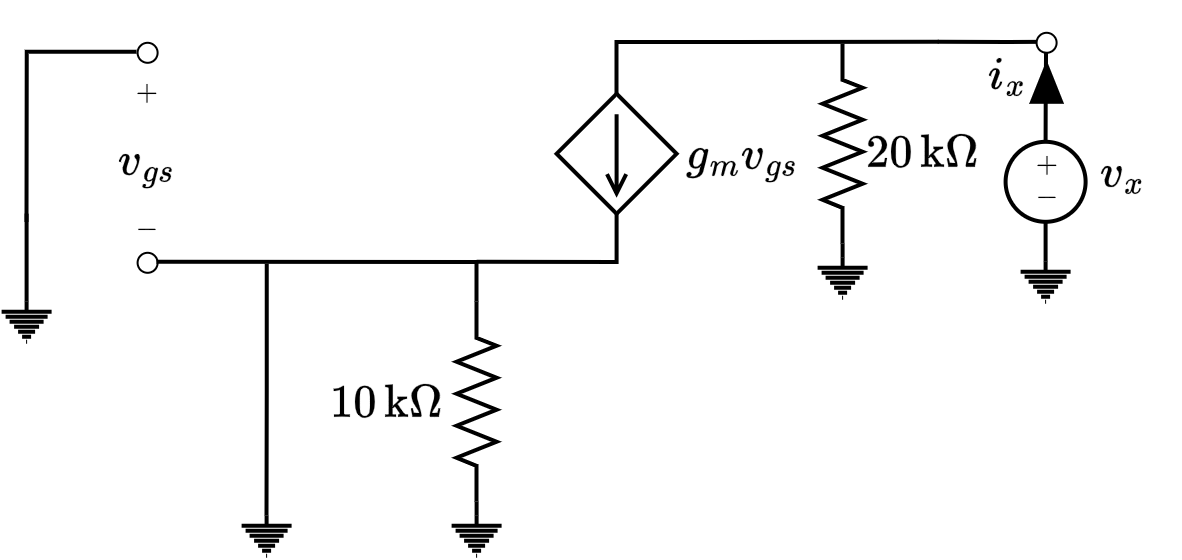
\includegraphics[width=4.5in]{sscg2.png}
\end{center}

From this circuit we can see that $v_{gs}=0$, so the dependent current source goes away.  Remember that we do not consider the load when calculating output resistance. It follows simply that:

\[ R_o = \qty{20}{\kilo\ohm}\]

\end{answer}
\end{partquestion}

\begin{partquestion}{overallgain}{Find the overall voltage gain $\frac{v_{o}}{v_{i}}$ if the output of the CD stage is connected to the input of the CG stage.}
\begin{answer}
The equivalent circuit of the cascaded amplifiers is shown below:

\begin{center}
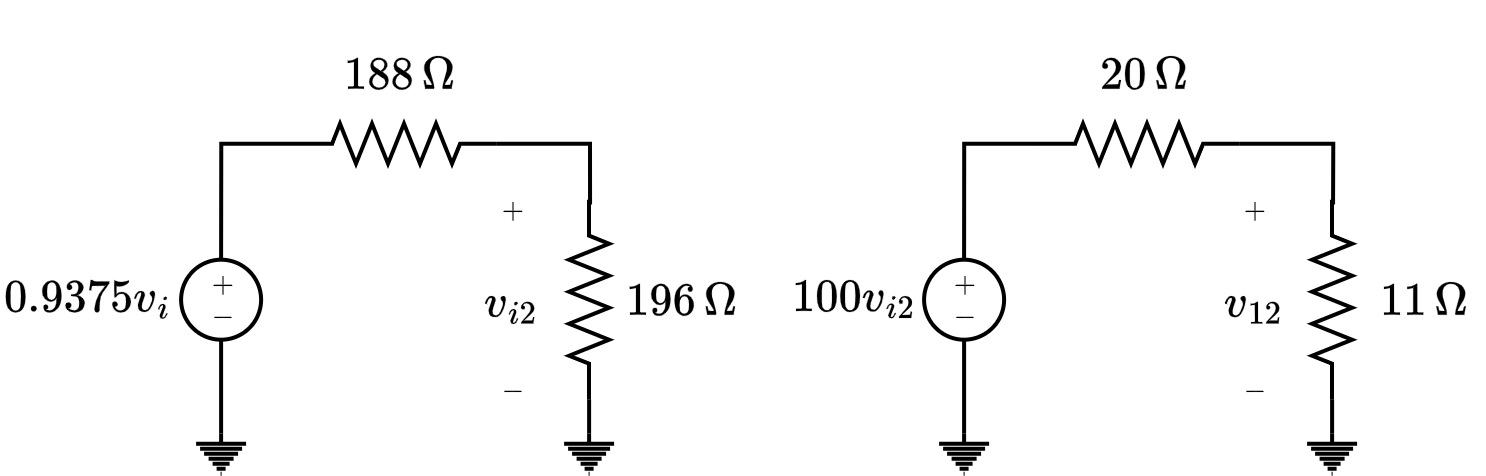
\includegraphics[width=4.5in]{model.png}
\end{center}

We can write:
\begin{align*}
    G_v &= \frac{v_o}{v_i} \\
    &= (0.9375)\frac{R_{i2}}{R_{o1} + R_{i2}}(100)\left(\frac{R_L}{R_{o2} + R_L}\right) \\
    &= (0.9375)\frac{196}{196 + 188}(100)\left(\frac{11}{11 + 20}\right) \\
    &= 16.98 \approx 17
\end{align*}

\end{answer}
\end{partquestion}

\end{mainquestion}
